\subsectionaddtolist{بررسی ارتباط از طریق Telnet}

در ابتدا نیاز است تا telnet را روی ویندوز فعال کنیم. وارد
 \lr{control panel}
 می‌شویم و در بخش Programs گزینه‌ی
\lr{Turn  Windows features on or off}
را انتخاب می‌کنیم.
سپس به دنبال 
\lr{telnet client}
می‌گردیم و آن را فعال می‌کنیم.



حال وارد cmd شده و با استفاده از دستور 
\lr{telnet telehack.com}
به آن متصل می‌شویم. البته قبل از آن باید wireshark‌ را در حالت capture بر روی interface اینترنت خود قرار دهیم. سپس تعدادی از دستورات را امتحان کرده و در نهایت capture را متوقف می‌کنیم.

در Wireshark فیلتر را روی
\lr{telnet}
قرار داده و بسته‌ها را مشاهده می‌کنیم:


{
	\centering{
		
		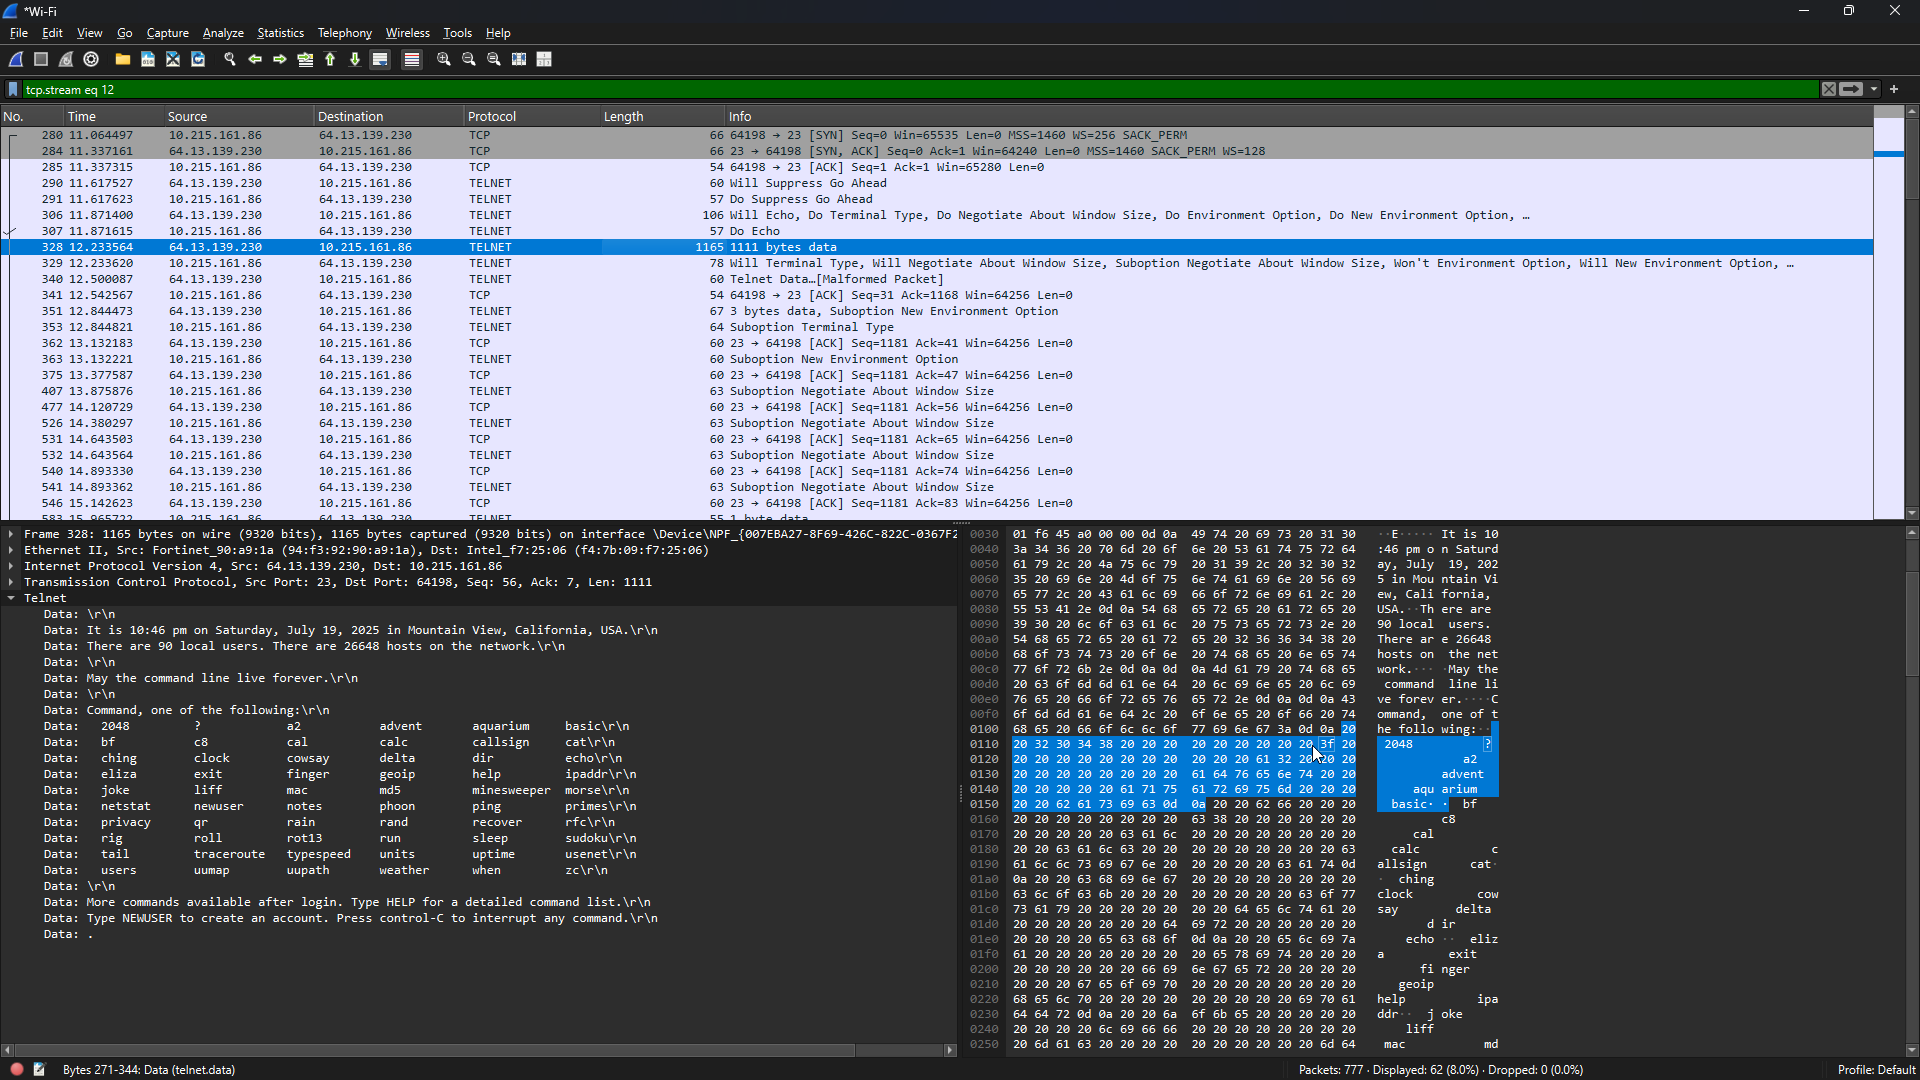
\includegraphics[width=1\textwidth]{screenshot001}
		
	}
}

به عنوان مثال این بسته مربوط به پیام welcome این سیستم است که دستورات خود را به ما معرفی کرده است.

برای این که پیام‌ها را دنبال کنیم، روی این بسته کلیک راست کرده و از منوی follow‌ گزینه‌ی 
\lr{tcp stream}
را انتخاب می‌کنیم.

{
	\centering{
		
		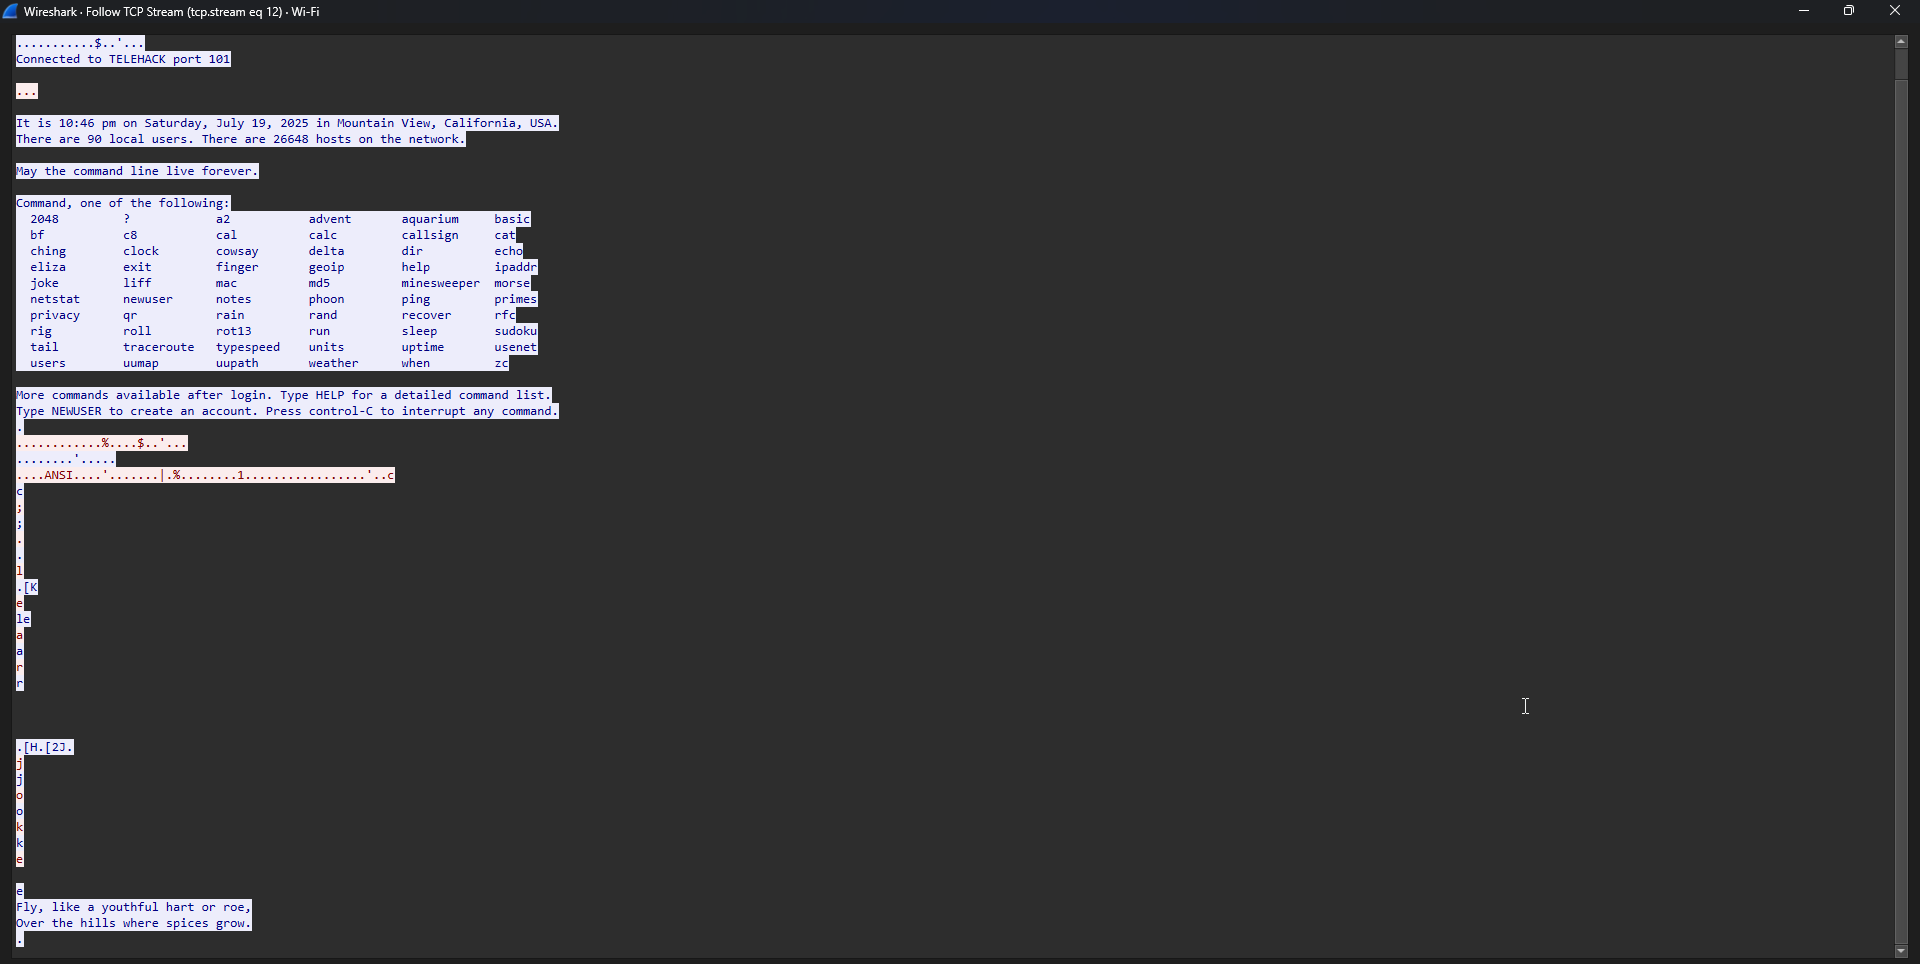
\includegraphics[width=1\textwidth]{screenshot002}
		
	}
}

همانطور که در تصویر مشخص است، من با استفاده از کامند 
\lr{joke}
درخواست یک جوک کردم و در اخرین بسته این جوک به دست من رسیده است.

نکته مهمی که در شل گرفتن قابل توجه است، این است که وقتی ما در شل تایپ می‌کنیم. هر کارکتر در یک بسته جدا به سمت سرور فرستاده می‌شود و سپس از سمت سرور اگر به درستی به دستش رسیده باشد همان را برای ما برمی‌گرداند. این موضوع داخل 
\lr{tcp trace}
فوق قابل مشاهده است.


نکته مهم دیگری که در این پروتوکل مورد توجه قرار می‌گیرد، این است که پیام‌ها و بسته‌ها به صورت رمزنگاری نشده رد و بدل می‌شود که نشان دهنده امنیت پایین‌تر این پروتوکل نسبت به پروتوکل‌های دیگر نظیر SSH است.

\subsubsection*{سوال ۱.}


{
	\centering{
		
		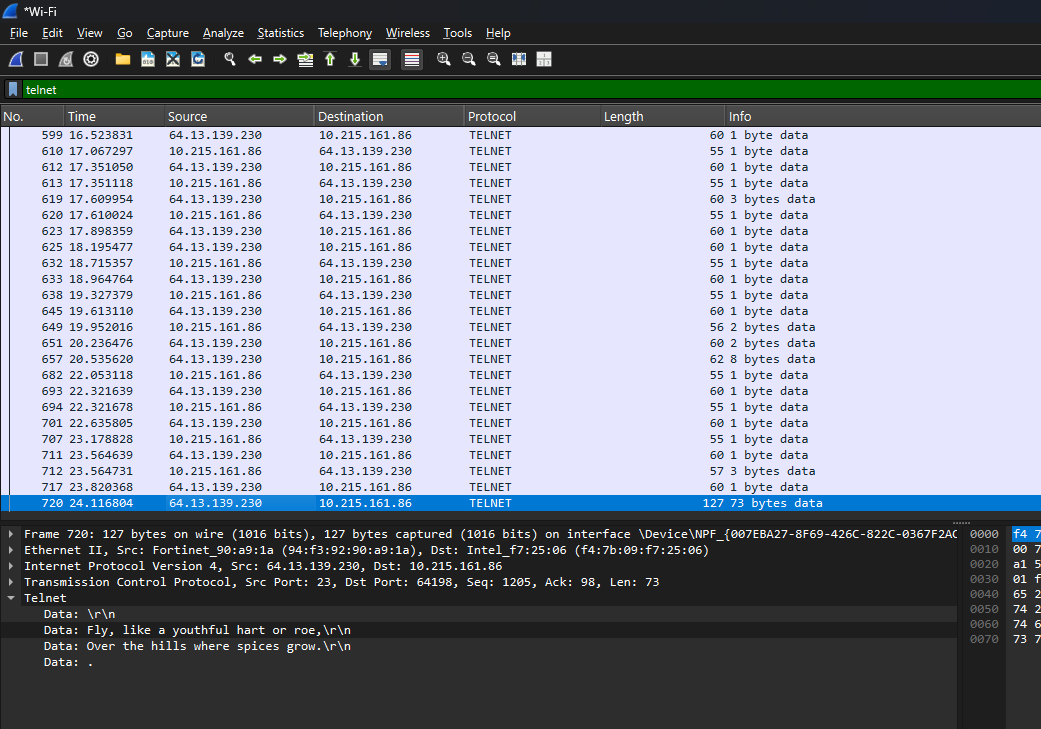
\includegraphics[width=0.7\textwidth]{screenshot003}
		
	}
}

با توجه به شکل فوق واضح است که آیپی سرور Source و ایپی من Destination است.

{
	\centering{
		
		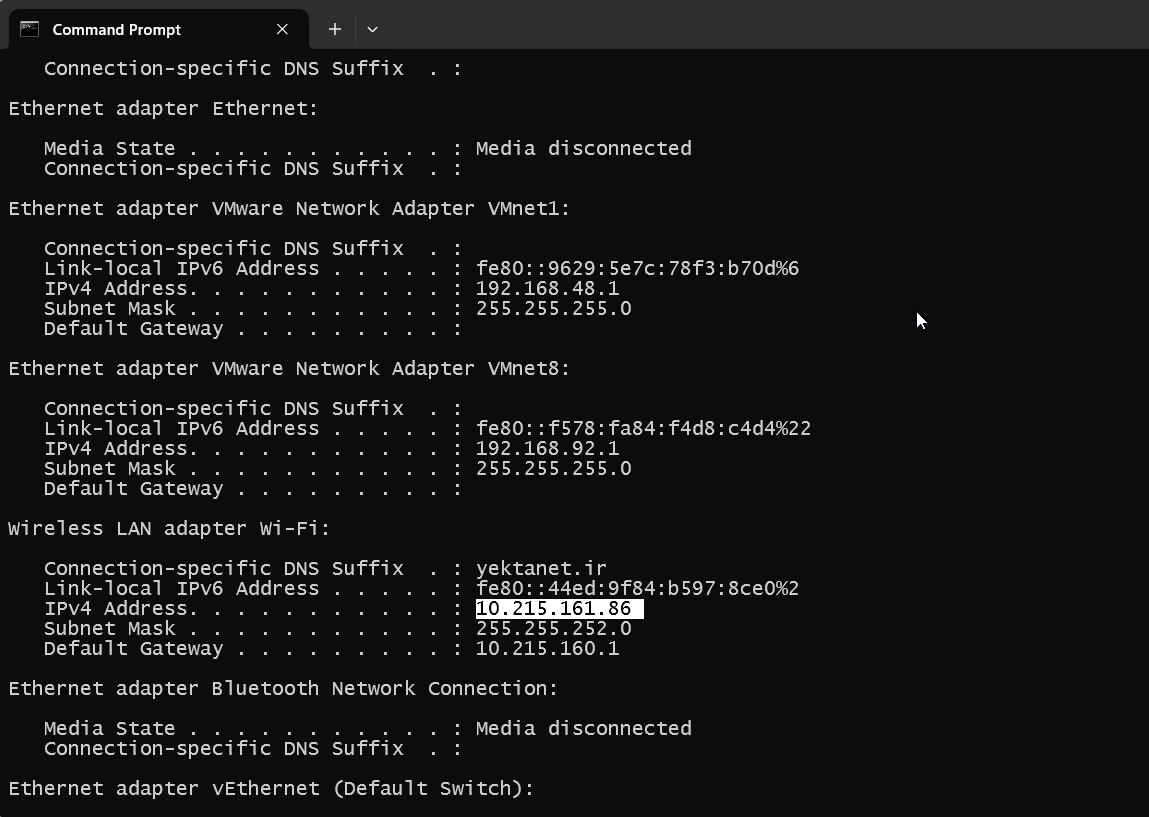
\includegraphics[width=0.7\textwidth]{screenshot004}
		
	}
}


برای اطمینان از صحت عملکرد، دستور 
\lr{ipconfig}
را در cmd وارد کرده و آیپی خود را مشاهده می‌کنیم.
\subsubsection*{سوال ۲.}

در این بخش هم با استفاده از 
\lr{tcp stream}
می‌توانیم بسته‌های مبادله شده را مشاهده کنیم. من به عنوان تست از یوزرنیم \lr{fake} و پسورد \lr{1234} استفاده می‌کنم.

{
	\centering{
		
		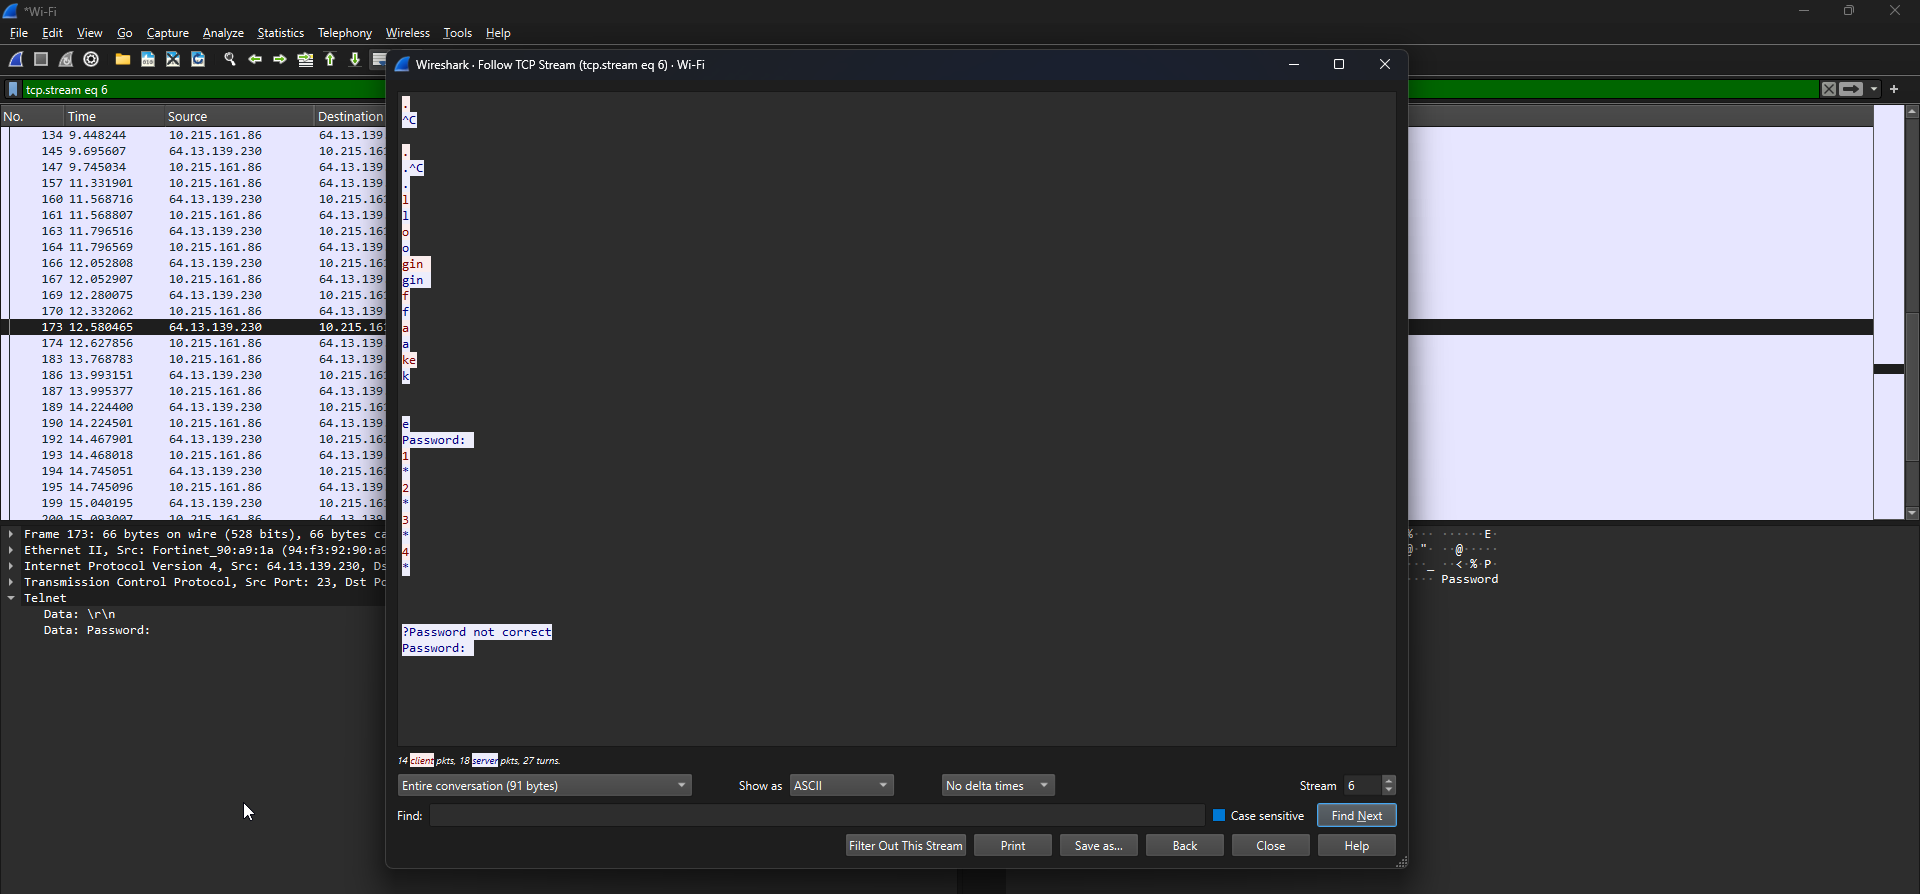
\includegraphics[width=1\textwidth]{screenshot005}
		
	}
}


همانطور که مشخص است پسورد و یوزرنیم به صورت raw بین کلاینت و سرور مبادله شده است و به راحتی قابل دسترسی است.


\pagebreak

\subsubsection*{سوال ۳.}


واضح است که بسته‌های آبی مربوط به من و بسته‌های قرمز مربوط به سرور است.

{
	\centering{
		
		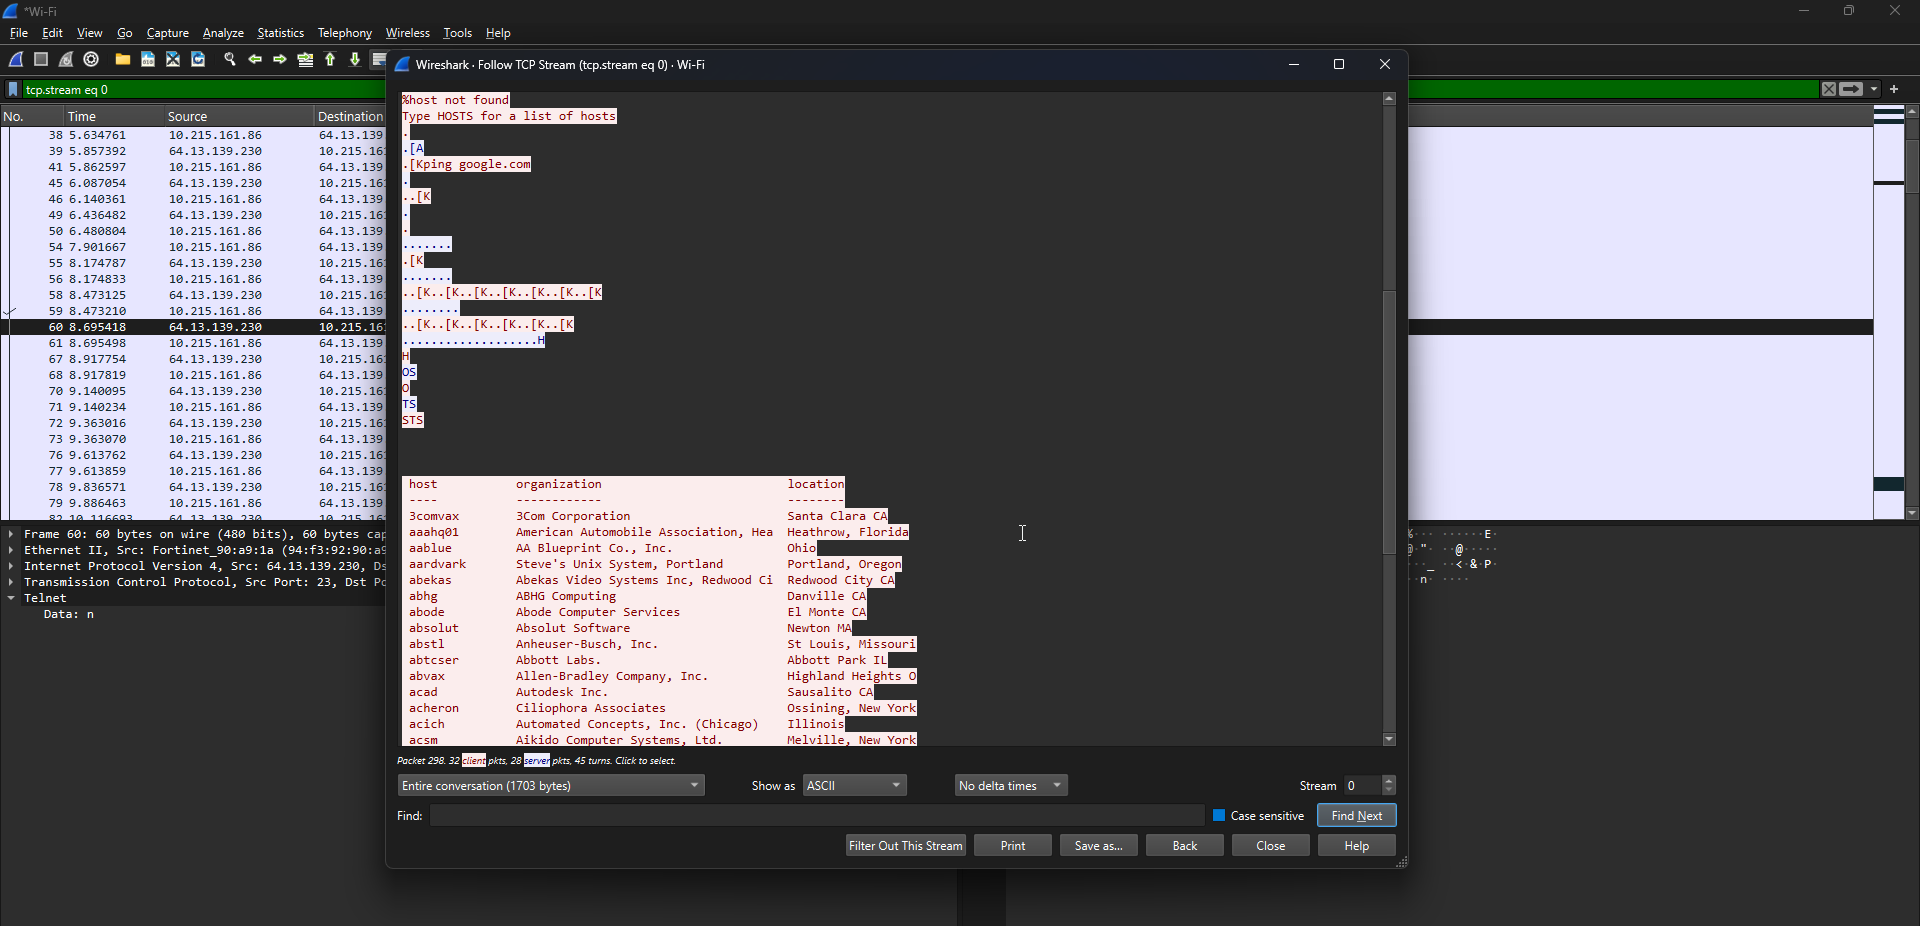
\includegraphics[width=1\textwidth]{screenshot006}
		
	}
}

